\section{\Glsfmtlong{asr}}

L'\gls{asr} est une autre branche du \gls{nlp}.
Son but est d'extraire automatiquement d'un signal audio qui représente une parole
la représentation textuelle de cette parole~\cite{Huang_Hayashi_Wu_Kameoka_Toda_2021}.

Les méthodes d'\gls{asr} peuvent être divisées en méthodes basées sur l'acoustique,
méthodes basées sur la reconnaissance de motifs
et méthodes basées sur l'intelligence artificielle (voir Figure~\ref{fig.asr-taxonomy-tree}).

\begin{figure}
    \centering
    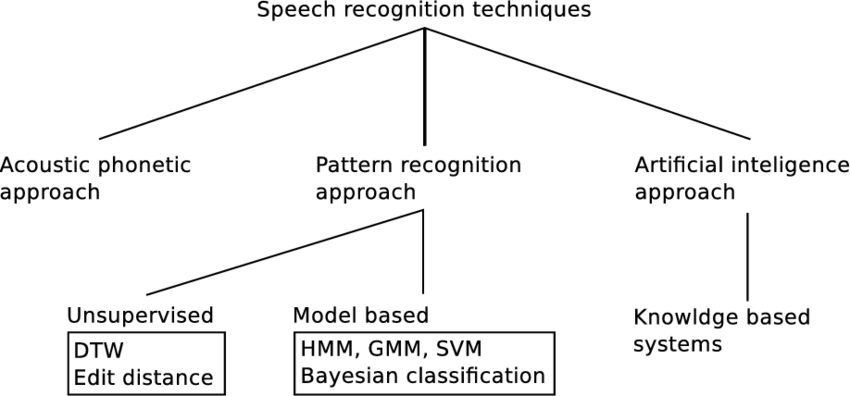
\includegraphics[width=\textwidth]{assets/images/Taxonomy-of-techniques-used-in-ASR.png}
    \caption[Taxonomie des techniques d'\gls{asr}.]
    {Taxonomie des techniques d'\gls{asr}~\cite{Volny_Novak_Zezula_2012}.}
    \label{fig.asr-taxonomy-tree}
\end{figure}

Comme pour la \gls{mt},
notre intérêt porte principalement sur les méthodes à base d'intelligence artificielle.
Plus spécifiquement sur les méthodes qui utilisent le \gls{dl}.